\documentclass[11pt, oneside]{article}   	% use "amsart" instead of "article" for AMSLaTeX format
\usepackage{geometry}                		% See geometry.pdf to learn the layout options. There are lots.
\usepackage{amsmath}

\geometry{letterpaper}                   		% ... or a4paper or a5paper or ... 
%\geometry{landscape}                		% Activate for for rotated page geometry
%\usepackage[parfill]{parskip}    		% Activate to begin paragraphs with an empty line rather than an indent
\usepackage{graphicx}				% Use pdf, png, jpg, or eps with pdflatex; use eps in DVI mode
								% TeX will automatically convert eps --> pdf in pdflatex		
\usepackage{amssymb}
\graphicspath{{/Users/telliott_admin/Dropbox/Tex/png/}}

\title{Rotation and reflection matrices for two dimensions}
%\author{The Author}
\date{}							% Activate to display a given date or no date

\begin{document}
\maketitle
\subsection*{rotation}
%\subsection{}
\large
\noindent
We begin by looking at the geometry of rotation of a point counter-clockwise.
\begin{center}
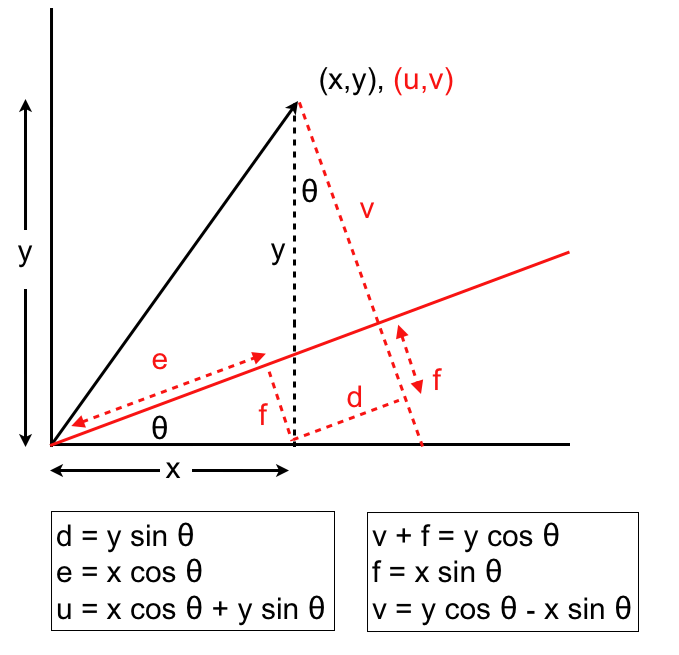
\includegraphics [scale=0.4] {ccw_rotation.png}
\end{center}
Looking at the diagram, we obtain equations for the new coordinates u,v in terms of the old coordinates x,y.  Rewriting this result using vector notation
\[
\begin{bmatrix}   \ \ \cos \theta & \sin \theta  \\  -\sin \theta & \cos \theta  \end{bmatrix}
\begin{bmatrix}   x   \\  y  \end{bmatrix} = \begin{bmatrix}   u   \\  v  \end{bmatrix}
\]
If we write  the multiplication explicitly we have
\[
u = x \cos \theta + y \sin \theta
\]
\[
v = -x \sin \theta + y \cos \theta
\]
The matrix for clockwise rotation can also be obtained by a geometric construction, but since we already have the equations just mutliply u and v by sine and cosine as follows
\[
u \sin \theta = x \sin \theta \cos \theta + y \sin^2 \theta
\]
\[
v \cos \theta = -x \sin \theta \cos \theta + y \cos^2 \theta
\]
\[
y = u \sin \theta+ v \cos \theta
\]
By a similar process we obtain
\[
x = u \cos \theta - v \sin \theta
\]
Since x, y, u, and v are just "dummy" variables (we could use any letters), switch back to having x, y as the first vector and in vector notation we have (for clockwise rotation)
\[
\begin{bmatrix}   \cos \theta & -\sin \theta  \\  \sin \theta &\ \  \cos \theta  \end{bmatrix}
\begin{bmatrix}   x   \\  y  \end{bmatrix} = \begin{bmatrix}   u   \\  v  \end{bmatrix}
\]
To check this, set the angle to $90^\circ$, then the matrix for clockwise rotation is
\[
\begin{bmatrix}   0 & -1  \\  1 &\ \  0  \end{bmatrix}
\]
This matrix multiplied by x, y produces -y, x, which is correct.
We can check this a little further by computing the matrices for $\pi/3$, $\pi/4$ and $\pi/6$.  They are
\[ R_{\pi/3} =
\begin{bmatrix}   
\ 1/2 & -\sqrt{3}/2  \\  
\ \sqrt{3}/2 & 1/2
\end{bmatrix}, \ \ 
 R_{\pi/4} =
\begin{bmatrix}   
\ 1/\sqrt{2} & -1/\sqrt{2}  \\  
\ 1/\sqrt{2} & 1/\sqrt{2}
\end{bmatrix},  \ \
 R_{\pi/6} =
\begin{bmatrix}   
\ \sqrt{3}/2 & -1/2  \\  
\ 1/2 & \sqrt{3}/2
\end{bmatrix}
\]
Notice that 
\[
\begin{bmatrix}   
\ 1/\sqrt{2} & -1/\sqrt{2}  \\  
\ 1/\sqrt{2} & 1/\sqrt{2}
\end{bmatrix}
\begin{bmatrix}   
\ 1  \\  
\ 0
\end{bmatrix}
=
\begin{bmatrix}   
\ 1/\sqrt{2}  \\  
\ 1/\sqrt{2}
\end{bmatrix}
\]
Which is a $45^\circ$ ccw rotation.
And that $30^\circ$ (right matrix) followed by $60^\circ$ is indeed $90^\circ$.
\[
\begin{bmatrix}   
\ 1/2 & -\sqrt{3}/2  \\  
\ \sqrt{3}/2 & 1/2
\end{bmatrix}
\times
\begin{bmatrix}   
\ \sqrt{3}/2 & -1/2  \\  
\ 1/2 & \sqrt{3}/2
\end{bmatrix}
=
\begin{bmatrix}   
\ 0 & -1  \\  
\ 1 & 0
\end{bmatrix}
\]


\end{document}  